\documentclass[tikz, border=5pt]{standalone}
\usepackage{tikz}
\usetikzlibrary{arrows.meta, positioning}

\begin{document}

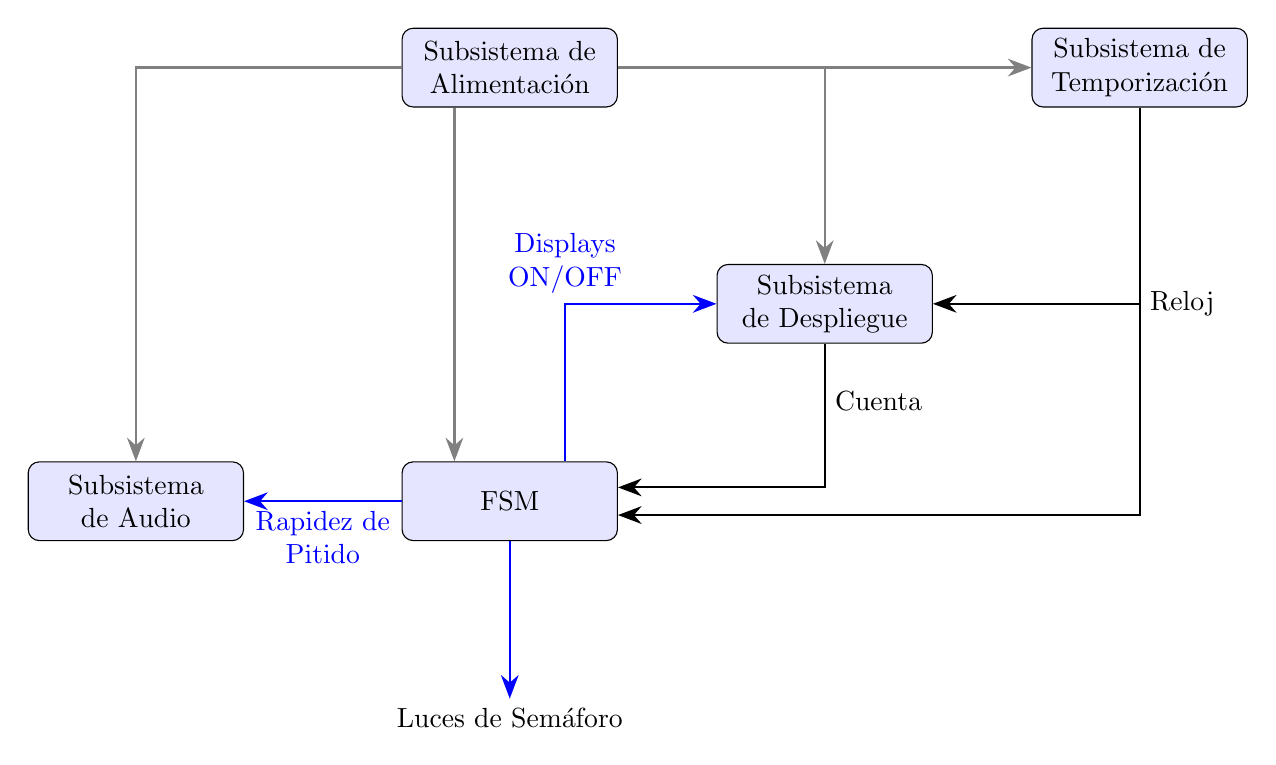
\begin{tikzpicture}[
    node distance=2cm,
    block/.style={rectangle, draw, fill=blue!10, text width=2.5cm, text centered, rounded corners, minimum height=1cm},
    arrow/.style={thick, -{Stealth[length=3mm]}}
]

\node (alimentacion) [block] at (0,0) {Subsistema de Alimentación};
\node (despliegue) [block] at (4,-3) {Subsistema de Despliegue};
\node (temporizacion) [block] at (8, 0) {Subsistema de Temporización};
\node (fsm) [block, below] at (0,-5) {FSM};
\node (audio) [block, left =of fsm] {Subsistema de Audio};

\node (luces) [below =of fsm] {Luces de Semáforo};

\draw [arrow, gray] (alimentacion) -- (temporizacion);
\draw [arrow, gray] (alimentacion) -| (despliegue);
\draw [arrow, gray] (alimentacion) -| (audio);
\draw [arrow, gray] ([xshift=-20pt]alimentacion.south) -- ([xshift=-20pt]fsm.north);

\draw [arrow] (temporizacion) |- node[right] {Reloj} (despliegue);
\draw [arrow] (temporizacion) |- ([yshift=-5pt]fsm.east);

\draw [arrow, blue] (fsm) -- node[below] {\shortstack{Rapidez de \\ Pitido}} (audio);
\draw [arrow, blue] ([xshift=20pt]fsm.north) |- node[above] {\shortstack{Displays \\ ON/OFF}} (despliegue.west);
\draw [arrow, blue] (fsm) -- (luces);

\draw [arrow] (despliegue) |- node[pos=0.2, right] {Cuenta} ([yshift=5pt]fsm.east);
\end{tikzpicture}

\end{document}
